\documentclass[10pt]{beamer}
%\documentclass[10pt, handout]{beamer}
\setbeameroption{show notes}

%\documentclass[10pt, a4paper]{article}
%\usepackage{beamerarticle}




\mode<article>{
	
	\usepackage{hyperref}
	
}
\mode<presentation>{
	
	\usetheme{Antibes}
	\usefonttheme{professionalfonts} 
	\usefonttheme{serif} % default family is serif
	
	%\usecolortheme{spruce} %зеленая, плохой цвет в заголовках 
	%\usecolortheme{albatross} %синяя, пхоло виден черный цвет
	
}

\newcommand{\MP}[1]{\mode<presentation>{#1} }
\newcommand{\MA}[1]{\mode<article>{#1} }

\newcommand{\ABS}[1]{\left| #1 \right|}
%\newcommand{\ABS}[1]{\mid #1 \mid}

\newcommand{\HREF}[2]{{\color{blue}\underline{\href{#1}{#2}}}}

\setbeamertemplate{caption}[numbered]


%\usepackage[T2A]{fontenc}
%\usepackage[utf8]{inputenc}
%\usepackage[russian]{babel}
%\usepackage{amsmath} %математические формулы



\usepackage{ifthen}

\usepackage{tikz}
\usetikzlibrary{arrows.meta}
\usetikzlibrary{calc}
\usetikzlibrary{decorations}
\usetikzlibrary{decorations.pathreplacing}
\newcommand{\rememb}[1]{\tikz[remember picture,baseline=-0.5ex]{\draw node[inner sep=0pt, outer sep=0pt] (#1){\strut};}}



\usepackage{fp}
\usepackage{tikz-3dplot}
\usepackage{environ}
\usepackage{animate}





\usepackage{xcolor}
%\usepackage[left=20mm,right=20mm,top=20mm,bottom=20mm,a4paper]{geometry} %поля

\usepackage{amsmath} %математические формулы
%\usepackage{amsfonts} %математические шрифты


\usepackage[e]{esvect}  %Красивая стрелочка вектора
%\let\oldvv\vv
\newcommand{\VV}[1]{\vv{#1\mathstrut}}



\usepackage{graphicx} %работа с каритнками


%\usepackage{multimedia}
%\usepackage{movie15}

%Для XeLatex/+
\usepackage{polyglossia}
\setdefaultlanguage{russian}
\setotherlanguage{english}
%\setkeys{russian}{babelshorthands=true} 


\usepackage{fontspec}

\setmainfont{Times New Roman} [Script=Cyrillic, Mapping=tex-text,]
\setsansfont{Arial} [Script=Cyrillic, Mapping=tex-text,]
%\setmonofont{Courier New} [Script=Cyrillic, Mapping=tex-text,]
\newfontfamily{\cyrillicfonttt}{Courier New}


%\usepackage{unicode-math}
%\setmathfont{TeX Gyre Termes Math}

%\setmainfont{CMU Serif}[Script=Cyrillic, Mapping=tex-text,]
%\setsansfont{CMU Sans Serif}[Script=Cyrillic, Mapping=tex-text,]
%\setmonofont{CMU Typewriter Text}[Script=Cyrillic, Mapping=tex-text,]


%-----------------


%\usepackage{caption}
%\DeclareCaptionLabelSeparator{dot}{~---~}            %Разделитель номер рисунка
%\captionsetup[figure]{justification=centering,labelsep=dot, format=plain}                        %Подпись рис. центр
%\captionsetup[table]{justification=raggedleft,labelsep=dot, format=plain, singlelinecheck=false} %Подпись табл. слева
%\captionsetup[lstlisting]{justification=raggedleft,labelsep=dot, format=plain, singlelinecheck=false}                     %Подпись рис. центр

\usepackage{indentfirst} %отступ первой строки


\usepackage[svgnames]{xcolor}


\usepackage{hyperref}

%\usepackage{showframe}


%\usepackage{tikz}

%\usepackage[hidelinks]{hyperref}%ссылки внутри документа \ref


\setlength\abovecaptionskip{-2pt}
%\setlength\belowcaptionskip{-14pt}

\setbeamerfont{caption}{size=\scriptsize}


\def\sectionname{Раздел}
\def\subsectionname{Подраздел}


\newcommand{\TC}[3]
{
	
	
	\begin{columns}
		\begin{column}{#1\textwidth}
			#2
		\end{column}
		\begin{column}{\fpeval{1-#1}\textwidth}
			#3
		\end{column}
	\end{columns}
}

\newcommand{\TCT}[3]
{
	
	\begin{columns}[T]
		\begin{column}{#1\textwidth}
			#2
		\end{column}
		\begin{column}{\fpeval{1-#1}\textwidth}
			#3
		\end{column}
	\end{columns}
}


\newcommand{\FRAME}[2]{
	\begin{frame}
		\frametitle{#1}
		#2
	\end{frame}
}

\newcommand{\FIG}[3]
{
	\begin{figure}
		\centering
		\includegraphics[width=#3]{#1}
		\caption{#2}
	\end{figure}
}

\newcommand{\vect}[1]{\overrightarrow{#1}}


\usepackage{qrcode}

\newcommand{\LECADDR}{https://clck.ru/3D3Efj}


\usepackage{newfile}

\edef\LectionNumber{0}
\edef\LectionTheme{0}

\let\oldsection\section
\let\oldsubsection\subsection


\AtBeginDocument
{
	\newoutputstream{CONTENT}
	\openoutputfile{\LectionNumber .gvr}{CONTENT}
	
	\expandafter\addtostream{CONTENT}{\noindent\textbf{\Large Лекция \LectionNumber~---~\LectionTheme}\unexpanded{\setcounter{SEC}{0}}\par}
}

\renewcommand{\section}[1]{
	\oldsection{#1}
	\expandafter\addtostream{CONTENT}{\noindent\hspace{2ex}\unexpanded{\hbox{\large\stepcounter{SEC}\theSEC ~ #1}}\par}
}

\renewcommand{\subsection}[1]{
	\oldsubsection{#1}
	\expandafter\addtostream{CONTENT}{\noindent\hspace{6ex}\unexpanded{\stepcounter{SUB}\theSUB ~ #1}\par}
}


%\renewcommand{\section}[1]{\MMM{#1}}

%\edef\subsection#1
{
	%\noexpand\subsection{#1}
	%
}


\newfontfamily\dnifamily[Scale = 0.795]{DniFont.TTF}

\newcommand{\dni}[1]{%
	{\dnifamily%
		\ifthenelse{#1=0}{0}{}%
		\ifthenelse{#1=1}{1}{}%
		\ifthenelse{#1=2}{2}{}%
		\ifthenelse{#1=3}{3}{}%
		\ifthenelse{#1=4}{4}{}%
		\ifthenelse{#1=5}{5}{}%
		\ifthenelse{#1=6}{6}{}%
		\ifthenelse{#1=7}{7}{}%
		\ifthenelse{#1=8}{8}{}%
		\ifthenelse{#1=9}{9}{}%
		\ifthenelse{#1=10}{)}{}%
		\ifthenelse{#1=11}{!}{}%
		\ifthenelse{#1=12}{@}{}%
		\ifthenelse{#1=13}{\#}{}%
		\ifthenelse{#1=14}{\$}{}%
		\ifthenelse{#1=15}{\%}{}%
		\ifthenelse{#1=16}{\^{}}{}%
		\ifthenelse{#1=17}{\&}{}%
		\ifthenelse{#1=18}{*}{}%
		\ifthenelse{#1=19}{(}{}%
		\ifthenelse{#1=20}{[}{}%
		\ifthenelse{#1=21}{]}{}%
		\ifthenelse{#1=22}{\textbackslash{}}{}%
		\ifthenelse{#1=23}{\{}{}%
		\ifthenelse{#1=24}{\}}{}%
		\ifthenelse{#1=25}{|}{}}%
}%

\newcommand{\toDni}[1]{%	
	\ifthenelse{#1=0}{}{%
		 \ifthenelse{#1=25}{%
		 	\expandafter\dni{#1}}{%
		 	\expandafter\toDni{\fpeval{floor(#1/25)}}%
		 \expandafter\dni{\fpeval{(#1/25 - floor(#1/25))/0.04}}}}%
}%



\newcommand{\Strut}{{\Large\strut}}

\newcommand\scb[1]{\left( #1 \right)}

\newcommand{\LINK}[2]{%
	\qrcode[height=1cm]{#1}\  \HREF{#1}{\parbox{0.8\textwidth}{#2}} \\[0.5em]
}

\NewDocumentCommand{\lecdni}{}{\toDni{\LectionNumber}}
\author{Гаврилов Андрей Геннадьевич}
\newcommand{\regals}{кандидат технических наук, доцент}
\institute{Кафедра Информационных технологий и вычислительных систем \\МГТУ~<<СТАНКИН>>}
\lecture{История компьютерной графики}{kghistory}\subtitle{Компьютерная графика}


\makeatletter
\newcommand*{\overlaynumber}{\number\beamer@slideinframe}
\makeatother



\usepackage{cprotect}

\newcommand{\QRFRAME}{%
    \begin{frame}[plain, noframenumbering]    	
	
	\centering
	Трансляция презентации (во время очных лекций)    
	
	~
	
	{\Large \ttfamily  https://clck.ru/3D3Efj  }
	
	~
	
	\tikz\node[inner sep=0pt,rounded corners=5mm, clip]{\qrcode[height=0.45\textwidth]{\LECADDR}}; 
	
	~	
	{\small
	При просмотре презентации в PDF для отображения анимаций на слайдах необходимо использовать Acrobat Reader, KDE Okular, PDF-XChange, Foxit Reader, браузер Firefox. Для браузеров на движке Chrome (Edge, Яндекс, Opera,~\dots) необходимо использовать \HREF{https://chromewebstore.google.com/detail/pdf-viewer/oemmndcbldboiebfnladdacbdfmadadm?hl=ru&utm_source=ext_sidebar}{PDF.js} c опцией <<Enable active content (JavaScript) in PDFs>>. }
	
	\end{frame}%
}

\newcommand{\IG}[2][1]{\includegraphics[width=#1\textwidth]{#2}}



\graphicspath{{Images/}{Images/\jobname/}}

\date{\today}


\renewcommand{\LectionNumber}{5}
\renewcommand{\LectionTheme}{Операции с вершинами в графическом конвейере OpenGL}
\title{Лекция \lecdni \\ \LectionTheme}
\subtitle{Компьютерная графика}

%\usepackage{standalone}

\setbeamersize
{
	text margin left=0.5cm,
	text margin right=0.5cm
}

\usepackage{comment}


%	\transduration{2}
%   \transfade

 \begin{document}
 		 
	\makeatletter
\defbeamertemplate*{title page}{my theme}
{
	
	\hfill
	
	\begin{beamercolorbox}[wd=.9\paperwidth,center,]{title}%
		
	\end{beamercolorbox}%	
	
	\vbox to 1em {}
	
	\begin{beamercolorbox}[wd=.9\paperwidth,center,]{title}%
		\usebeamerfont{subtitle}%
		\hfill
		
		\insertsubtitle
		
		\usebeamerfont{title}%
		\inserttitle{} \\[0.5em]
		
		
		
	\end{beamercolorbox}%	
	\hfill\hfill
	
	\begin{beamercolorbox}[wd=.9\paperwidth,center,]{}%
		\usebeamerfont{author}%
		\hfill \\[0.5em]
		\insertauthor{} \\[0.5em]
		\regals
		    
		\vbox to 1em{}
		\usebeamerfont{institute}%
		\insertinstitute {}
		
		\vbox to 1em{}			
		{\; }\insertshortdate{}
		
	\end{beamercolorbox}%	
	\hfill\hfill
	
	\vbox to 5em{}
	
	
}
\defbeamertemplate*{footline}{my theme}{
	\leavevmode%
	\hbox{%
		\begin{beamercolorbox}[wd=.25\paperwidth,ht=3.25ex,dp=0ex,center,sep=1pt]{author in head/foot}%
			\usebeamerfont{author in head/foot}%
			\insertauthor 
			\beamer@ifempty{\insertshortinstitute}{}
		\end{beamercolorbox}%
		\begin{beamercolorbox}[wd=.65\paperwidth,ht=3.25ex,dp=0ex,center,sep=1pt]{title in head/foot}%
			\usebeamerfont{title in head/foot}\insertshortinstitute
		\end{beamercolorbox}%
		\begin{beamercolorbox}[wd=.1\paperwidth,ht=3.25ex,dp=0ex,center, sep=0.5pt]{date in head/foot}%
			\usebeamerfont{date in head/foot}
			\footnotesize \expandafter\toDni{\insertframenumber} / \expandafter\toDni{\inserttotalframenumber}
	\end{beamercolorbox}}%
}



\makeatother






%float page top aligment
\makeatletter
\setlength{\@fptop}{0pt}
\setlength{\@fpbot}{0pt plus 1fil}
\makeatother

\everymath{\displaystyle}

\begin{comment}

\end{comment}

    
    \QRFRAME
	
	
	\frame{\maketitle}
	
	
	
	\begin{frame}{План лекции}
		\tableofcontents
	\end{frame}
	
	\begin{frame}{Класический конвейер OpenGL}
		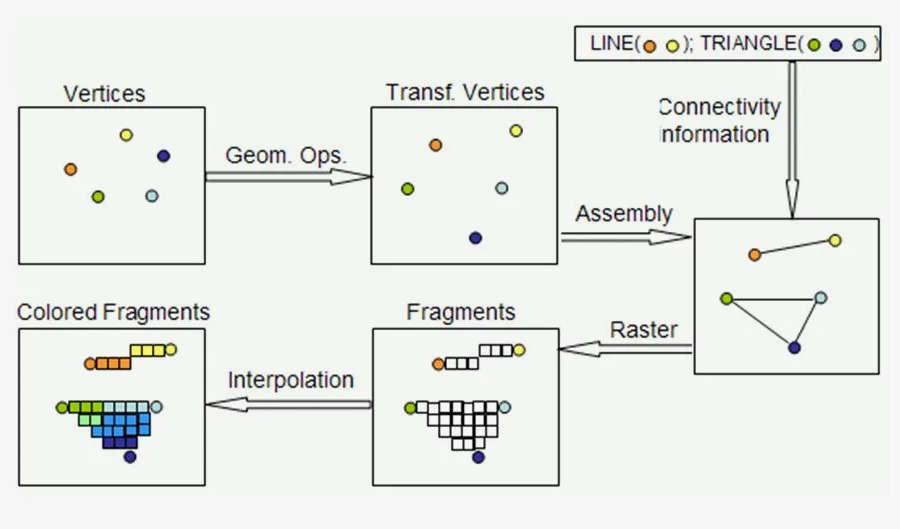
\includegraphics[width=\textwidth]{old_pipeline.png}
	\end{frame}
	
	
	\section{Вершинные операции. Преобразование координат  }
	
	\frame{\sectionpage}
	
	
	\subsection{Основная задача}
	
	\begin{frame}{Цель вершинных операций}
		\TCT{0.5}
		{
			\centering
			\textbf{У нас есть} объект в пространстве
			
			\fbox{\includegraphics{projectionPL_3.pdf}}
		}
		{
			\centering
			\textbf{А нам надо} объект на экране
			
			\fbox{\includegraphics{projectionPL_1.pdf}}
		}
	\end{frame}
	
	\begin{frame}{Системы координат сцены}
		\TCT{0.55}
		{
			\includegraphics{projectionPL.pdf}
		}
		{
			$x^My^Mz^M$  --- С.К. модели
			
			$xyz$  --- мировая С.К.
			
			$x^Vy^Vz^V$  --- С.К. наблюдателя (видовая) \\ ~ \\
			
			$\mathbf V^M
			=
			\begin{pmatrix}
				0.5 & -0.5 &-0.5& 0.5 &0\\
				0.5& 0.5 & 0.5 &-0.5& 0 \\
				0 &  0 &  0.5 &   0 & 0.4
			\end{pmatrix} $\\ ~ \\ ~ \\ 
			
			Задача:
			
			Получить координаты объекта $V^M$ в видовой СК: \\
			
			$V^M \rightarrow V \rightarrow V^V$ \\ ~ \\
			
			
		}
		
	\end{frame}
	
	\subsection{Мировые координаты}
	
	\begin{frame}{Расчёт мировых координат}
		Система координат модели $V$ определяется \fbox{\emph{модельной матрицей }  $\mathbf M^M$}. \\ 
		$\mathbf M^M$  --- совокупность трансформаций объекта, выраженных матрицами $\mathbf T(\vv p)$, $\mathbf R(\vv v, \theta)$, $\mathbf S(s_x,s_y,s_z)$, т.е. --- совокупность переносов, поворотов и масштабирований. \\ ~ \\
		
		\textbf{Пример:}
		\TC{0.5}{$\mathbf M^M = \mathbf T(1,3,5)\mathbf R_x(32^\circ)\mathbf R_z(-45^\circ) $}
		{
			Порядок действий (обратный записи):\\
			1. Поворот вокруг $z$ на -45$^\circ$.\\
			2. Поворот вокруг $x$ на 32$^\circ$.\\
			3. Перенос на $(1,3,5)$.\\
		}  ~ \\		
		
		\begin{block}{Переход в мировую С.К.}
			$$
			V^M \rightarrow V: \ \mathbf V = \mathbf M^M \mathbf V ^M
			$$
		\end{block}
		
	\end{frame}
	
	\subsection{Видовые координаты}
	
	\begin{frame}{Расчёт видовых координат}
		Видовая система координат определяется \fbox {видовой матрицей $\mathbf M^V$}. Центр видовой С.К. можно интерпретировать как положение наблюдателя сцены (камеры):
		 \begin{itemize}
		 	\item Наблюдатель смотрит в направлении \ $-z^V$.
		 	\item Ось $y^V$ --- направление наверх для наблюдателя.
		 \end{itemize}
		 
		 Положение камеры определяется комбинаций перемещений и поворотов, которые составляют $\mathbf M^V$. 
		 
		 \begin{block}{Переход в видовую С.К.}
		 	$$
		 	V \rightarrow V^V: \ \mathbf V^V = \mathbf M^V \mathbf V
		 	$$
		 \end{block}
		  
	\end{frame}
	
	
	\begin{frame} {Видовая матрица. Способ получения 1.}
		
		\TC{0.45}
		{
			\hbox to -0.5cm{}\includegraphics[page=2]{camera.pdf}
		}
		{
			Положение камеры определяется совокупностью перемещений и поворотов, которые поместили её туда, где она располагается:
			
			$ \mathbf M = \mathbf T(\dots)\mathbf R(\dots)\mathbf T(\dots)\dots $ \\~\\
			
			Задача сводится с переходу $xyz \rightarrow x^Vy^Vz^V $:
			
			$\mathbf A^V = \mathbf M^{-1}\mathbf A$ \\ ~ \\
			
			$ \mathbf M^{-1} = \mathbf M^V$ --- видовая матрица. \\ ~ \\
			
			или
			
			$\mathbf M^V =  \mathbf T^{-1}(\dots)\mathbf R^{-1}(\dots)\mathbf T^{-1}(\dots)\dots  $
			
		}
	\end{frame}
	
	\begin{frame}{Видовая матрица. Способ получения 2.}
		\TC{0.5}
		{
			\hbox to -1cm{}\includegraphics[page=1]{camera.pdf} \\
			
			Задача сводится к переходу от базиса $[ 
			    {\color{red}\vv i}  , 
				{\color{green}\vv j }, 
				{\color{blue}\vv k} 
				]$
				к 
				$[ 
				{\color{orange}\vv r},
				{\color{lime!80!black} \vv u} , 
				{\color{cyan} -\vv f} ]$ и сдвигу на $(-\vv e)$
		}
		{
			Камера располагается в координате $\vv e$. Направлена на т. $A$.
			
			Можно определить следующие единичные вектора:
			\begin{itemize}
				\item {\color{cyan}$\vv f$} --- направление на объект. 
				\item {\color{lime!80!black}$\vv u$} ---направление <<наверх>> для наблюдателя.
				\item {\color{orange}$\vv r$} ---направление <<направо>> для наблюдателя.
			\end{itemize}
			
			$\mathbf M^V = 
			\begin{pmatrix}
				{\color{orange}r_x} & {\color{lime!80!black}u_x} & {\color{cyan}-f_x}& -e_x \\
				{\color{orange}r_y} & {\color{lime!80!black}u_y} & {\color{cyan}-f_y}& -e_y \\
				{\color{orange}r_z} & {\color{lime!80!black}u_z} & {\color{cyan}-f_z}& -e_z \\
				0&0&0&1
			\end{pmatrix}$
						
		}
	\end{frame}
	
	\begin{frame} {Настройка камеры}
		
	\TC{0.46}
	{
		\hbox to -1.2cm{}\includegraphics[page=3]{camera.pdf}
	}
	{
		Исходные данные (подчёркнуты на рис.):
		\begin{itemize}
			\item Куда смотрим --- $A$.
			\item Откуда смотрим --- $e$
			\item Где небо --- ${\color{olive}\vv {up}}$.
		\end{itemize}
		Найти:  $	{\color{orange}\vv r},
		{\color{lime!80!black} \vv u} , 
		{\color{cyan} \vv f} $. \\ ~ \\
		
		
		1. $\vv f' = \vv A - \vv e,\ {\color{cyan} \vv f }= \vv f' / |\vv f'|$ \\ ~ \\ \pause
		
		2. $\vv{up}' = {\color{olive}\vv {up}} / |{\color{olive}\vv {up}}|, \ {\color{orange}\vv r} = {\color{cyan} \vv f }\times \vv {up}'$ \\ ~ \\ \pause
		
		3. ${\color{lime!80!black}\vv u} = {\color{orange}\vv r} \times {\color{cyan}\vv f}$ \\ ~ \\ 
		
		$\mathbf M^V = 
		\begin{pmatrix}
			{\color{orange}r_x} & {\color{lime!80!black}u_x} & {\color{cyan}-f_x}& -e_x \\
			{\color{orange}r_y} & {\color{lime!80!black}u_y} & {\color{cyan}-f_y}& -e_y \\
			{\color{orange}r_z} & {\color{lime!80!black}u_z} & {\color{cyan}-f_z}& -e_z \\
			0&0&0&1
		\end{pmatrix}$
		
	}
		
	\end{frame}
	
	\subsection{Команды управления матрицами в OGL}
	
	\begin{frame}{Преобразования в классическом OpenGL}
		
		\textbf{GL\_MODELVIEWMATRIX} --- константа обозначающая $\mathbf M^V \mathbf M^M$ (MV матрицу).
		
		\textbf{glGetFloatv(GL\_MODELVIEW\_MATRIX, ptr)} --- получить VM-матрицу в указатель ptr.
		
		\textbf{glMatrixMode(GL\_MODELVIEWMATRIX)} --- режим с VM-матрией. Команда говорит о том, что все дальнейшие матричные операции будут проводится с этой матрицей.
		
		\textbf{glLoadIdentity()}  --- установить единичную матрицу, сброс всех преобразований.
		
		\textbf{glMultMatrixd(ptr)} --- умножить текущую матрицу на матрицу в указателе ptr.
		
		\textbf{glLoadMatrixd(ptr)} --- установить текущую матрицу из указателя ptr.
		
		\textbf{glRotated($\dots$), glTranslated($\dots$), glScaled($\dots$)}  --- домножить матрицу на матрицы поворота, перемещения, масштабирования.
		
		\textbf{glPushMatrix(), glPopMatrix() }--- записать/считать матрицу из стека.
		
		\textbf{gluLookAt(ex,ey,ez,cx,cy,cz,ux,uy,uz)} --- настроить камеру с центром в $e$, смотрящую на $c$, небо по направлению $\vv{u}$.		
		
	\end{frame}
	
	\section{Вершинные операции. Проецирование}
	
	\frame {\sectionpage}
	
	\subsection{Канонический объём отсечения}
	
	\begin{frame}{Координатная система OpenGL}
		\TC{0.5}
		{
			\includegraphics[page=3]{cvv.pdf}
		}
		{
			Канонический объём отсечения или Canonic view volume (CVV) ---
			
			куб с ребром = 2 и центром в начале координат. \\~\\
			
			Грань куба $z^c=-1$ выступает в роли <<экрана>>. В кадр попадёт только то, что находится внутри куба, т.е. все точки у которых $|x^c|<1$,  $|y^c|<1$, $|z^c|< 1$.
		}
	\end{frame}
	
	
	\subsection{Перспективная проекция}
	
	\begin{frame}{А что мы видим?}
		\centering
		Видовая система координат и пространство отсечения при перспективной проекции
		
		\includegraphics[page=1, width=0.5\textwidth]{cvv_empty.pdf}
		
	\end{frame}
	
	
	\begin{frame}{Проекционное преобразование}
		
		\centering
		\begin{columns}
			\begin{column}{0.5\textwidth}
				\includegraphics[page=1,width=\textwidth]{cvv_empty.pdf}
			\end{column}
			
			\begin{column}{0.1\textwidth}
				$\Rightarrow$
			\end{column}
			
			
			\begin{column}{0.4\textwidth}
				\includegraphics[page=2,width=\textwidth]{cvv_empty.pdf}
			\end{column}
		\end{columns}
		
		
		
		
	\end{frame}
	
	
	\begin{frame} 
		\TC{0.5}
		{
			\includegraphics[width=\textwidth, page=1]{cvv.pdf}
		}
		{
		$z=-n$ --- ближняя плоскость отсечения
		
		$z=-f$ --- дальняя плоскость отсечения
		
		$w\times h$ --- ширина и высота <<экрана>> \\ ~ \\
		
		
		Исходя из этих параметров необходимо сконструировать матрицу преобразования вида:
		
		$ 
		\begin{pmatrix}
			a& 0& 0& 0 \\
			0 &b &0 &0 \\
			0 &0& c& d\\
			0& 0& -1& 0\\
		\end{pmatrix}
		\begin{pmatrix}
			x\\
			y\\
			z\\
			1
		\end{pmatrix}
		=
		$
		$
		=
		\begin{pmatrix}
			ax\\
			by\\
			cz+d\\
			-z
		\end{pmatrix}
		\Rightarrow
		\begin{pmatrix}
			-ax/z\\
			-by/z\\
			-(cz+d)/z\\
			1
		\end{pmatrix}
		$
		}
	\end{frame}
	
	\begin{frame}{}
		\begin{center}
			\includegraphics[page=4]{cvv.pdf}
		\end{center}
		
		
			$z^c = -(cz+d)/z$ \\
			
			$  
			\left\lbrace \begin{array}{rl}
				-1=	&(-cn+d) / n\\
				1 = &(-cf+d) / f\\
			\end{array}  
			\right.
			\Leftrightarrow
			\left\lbrace
			\begin{array}{l}
				\fbox{$c = (n+f) / (n-f)$} \\
				\tiny~\\
				\fbox{$d = 2fn / (n - f)$}
			\end{array}
			\right.
			$ 
		
		
		
		
	\end{frame}
	
	\begin{frame}
		\TCT{0.6}
		{
			\includegraphics[page=2]{cvv.pdf}
		}
		{
			
			
			$y^c = \displaystyle\frac {y}  {h/2/n} $, \  
			$x^c = \displaystyle\frac {x}  {w/2/n} $ 
			\\ ~ \\
			
			
			$\frac{1}{h/2/n} = \ctg{\alpha/2}$	 \\~\\
			
			$\frac w h = \text{asp}$	
				\\ ~ \\[5em]
				
			
			$y_c  = y \ctg{(\alpha/2)}$
			
			$x^c = \frac x {\text{asp} \, h /2 /n } = x \frac{\ctg{(\alpha/2)}}{\text{asp}} $ \\~\\
			
			\fbox{$b=\ctg{(\alpha/2)}$} \\ ~ \\
			\fbox{$a=\frac{\ctg{(\alpha/2)}}{\text{asp}}$}
		
		}
	\end{frame}
	
	\begin{frame}
		
	\TC{0.5}
	{
		\includegraphics[page=8, width=\textwidth]{cvv.pdf}
	}
	{
		$\mathbf P =$ \\[1ex]
		\footnotesize
		$
		\begin{pmatrix}
		\frac{\ctg\left(\displaystyle\frac{\text{fovy}} {2}\right)}{\text{asp}} & 0 & 0 & 0 \\	
		0 & \ctg\left(\frac {\text{fovy}} {2}\right) & 0 & 0 \\
		0 & 0 & \frac {n+f}{n-f} & \frac {2fn}{n-f} \\
		0 & 0 & -1 & 0
		\end{pmatrix}
		$
	}
		
	\end{frame}
	
	
	
	\begin{frame}
		
		
		\TC{0.5}
		{
			\centering
			
			\animategraphics[autoplay,loop,palindrome, width=\textwidth, nomouse]{30}{Images/\jobname/cvv_anim}{1}{99}
		}
		{
			\centering
			
			\animategraphics[autoplay,loop,palindrome, width=0.55\textwidth, nomouse]{30}{Images/\jobname/cvv_anim}{101}{199}
			
			\animategraphics[autoplay,loop,palindrome, width=0.7\textwidth, nomouse]{30}{Images/\jobname/cvv_anim}{201}{299}
		}
	\end{frame}
	
	\begin{frame}{Изменение дальних и ближних плоскостей}
		\centering\animategraphics[autoplay,loop, nomouse, width=0.8\textwidth]{15}{Images/\jobname/clip_anim/ezgif-frame-}{005}{080}
		
	\end{frame}
	
	\begin{frame}{Ошибка теста грубины}
			
		\TC{0.75}
		{
		
			\includegraphics{depth.pdf}

		}{
		
		        $z^c = -\dfrac{cz+d}{z}$, где \\[0.3ex] 
		        
		        $c = \dfrac{n+f}{n-f}$,
		        
		        $d = \dfrac{2fn}{n-f}$
		        
		        ~
				
				{ \color{red} $n=1$\\$f=100$   }
				
				~
				
				{ \color{blue} $n=5$\\$f=100$   }
	
		}
		
	\end{frame}
	
	\subsection{Параллельная проекция}
	
	\begin{frame}{Параллельное проекционное преобразование}
		\centering
		\begin{columns}
			\begin{column}{0.6\textwidth}
				\includegraphics[page=9,width=\textwidth]{cvv.pdf}
			\end{column}
			
			\begin{column}{0.1\textwidth}
				\centering
				$\Rightarrow$
			\end{column}
			
			\begin{column}{0.3\textwidth}
				\centering
				\includegraphics[page=2,width=\textwidth]{cvv_empty.pdf}
			\end{column}
		\end{columns}
	\end{frame}
	
	\begin{frame}{Матрица параллельной проекции}
		
		\centering
		\includegraphics[page=4]{cvv.pdf}
		
		\TCT{0.45}
		{
			$\mathbf P =
			\begin{pmatrix}
				a& 0& 0& t_x \\
				0& b& 0& t_y \\
				0& 0& c& t_z \\
				0& 0& 0& 1 \\
			\end{pmatrix}
			$
			
			$z^c = cz+t_z $
			
			$ \left\lbrace
			\begin{array}{rcl}
				-1 &= & -cn + t_z \\
				1& = & -cf + t_z
			\end{array}
			 \right. \Leftrightarrow $
			 
			 $ \Leftrightarrow \left\lbrace
			 \begin{array}{rcl}
			 	c &  = & -2/(f-n) \\
			 	t_z& = & (f+n)/(f-n)
			 \end{array}
			 \right. $
		}
		{
			$\mathbf P =
			\begin{pmatrix}
				\frac{2}{r-l}& 0& 0& -\frac{r+l}{r-l} \\
				0& \frac{2}{t-b}& 0& -\frac{t+b}{t-b} \\
				0& 0& \frac{-2}{f-n}& -\frac{f+n}{f-n} \\
				0& 0& 0& 1 \\
			\end{pmatrix}
			$
		}
		

		
		
		
		
	\end{frame}
	
	

	
	\begin{frame}
		
			\TC{0.5}
		{
			\centering
			
			\animategraphics[autoplay,loop,palindrome, width=\textwidth, nomouse]{30}{Images/\jobname/cvv_anim}{1}{99}
		}
		{
			\centering
			
			Перспективная проекция
			
			\animategraphics[autoplay,loop,palindrome, width=0.6\textwidth, nomouse]{30}{Images/\jobname/cvv_anim}{201}{299}
			
			Параллельная проекция
			
			\includegraphics[page=10, width=0.6\textwidth]{cvv.pdf}
		}
		
	\end{frame}
	
	
	\subsection{Установка проекций в OGL}
	
	\begin{frame}{Проекционные преобразования в классическом OpenGL}
		
		\textbf{glMatrixMode(GL\_PROJECTIONMATRIX)} --- устанавливаем режим работы с матрицей проекции. После этого функции для работы с матрицами будут затрагивать именно её.
		
		\textbf{gluPerspective(fovy,asp,n,f)} --- установка матрицы перспективной проекции.
		
		\textbf{glOrtho(l,r,t,b,n,f)} --- установка матрицы параллельной проекции.
		
		\textbf{gluOrtho2D(l,r,t,b)} --- установка матрицы параллельной проекции с $n=-1$, $f=1$.
		
		
	\end{frame}
	
	
	\subsection{Порт просмотра}
	\begin{frame}{Порт просмотра (viewport)}
		\TC{0.5}
		{
			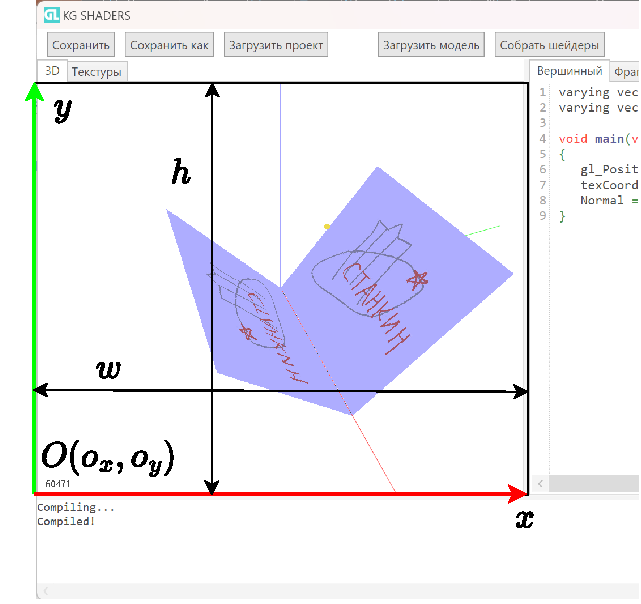
\includegraphics[width=\textwidth]{viewport.image.pdf}
		}
		{
			$(x^c,y^c) \rightarrow (x^{vp},y^{vp})$ \\ ~ \\
			
			$x^{vp} = (x^c+1)\frac{w}{2}+o_x$
			
			$y^{vp} = (y^c+1)\frac{h}{2}+o_y$ \\ ~ \\
			
			\textbf{glViewport(ox,oy,w,h)} --- установка вьюпорта.
			
			
		}
		
	\end{frame}
	
	\oldsection{Подведём итоги}
	
	\begin{frame}{Подведём итоги}
		
		\centering
		
		\includegraphics{itog.pdf}
		
		
	\end{frame}
	

\begin{comment}
\end{comment}

\end{document}